\documentclass[11pt]{standalone}
\usepackage{amssymb}
\usepackage{amsmath}
\usepackage[no-math]{fontspec}
\usepackage{unicode-math}
\usepackage{libertinus}
\usepackage{pgf,xcolor}
\usepackage{tikz}
\usetikzlibrary{arrows.meta, backgrounds, decorations.pathmorphing}
\usepackage{pgfplots}
\pgfplotsset{compat=newest}

\definecolor{my_darkgray}{HTML}{484949}
\definecolor{my_lightgray}{HTML}{F3F4F4}
\definecolor{my_darkblue}{HTML}{005A94}
\definecolor{my_lightblue}{HTML}{CCDEE9}
\definecolor{my_yellow}{HTML}{FFEC7F}
\definecolor{my_red}{HTML}{E60000}
\definecolor{my_orange}{HTML}{E87846}

\begin{document}
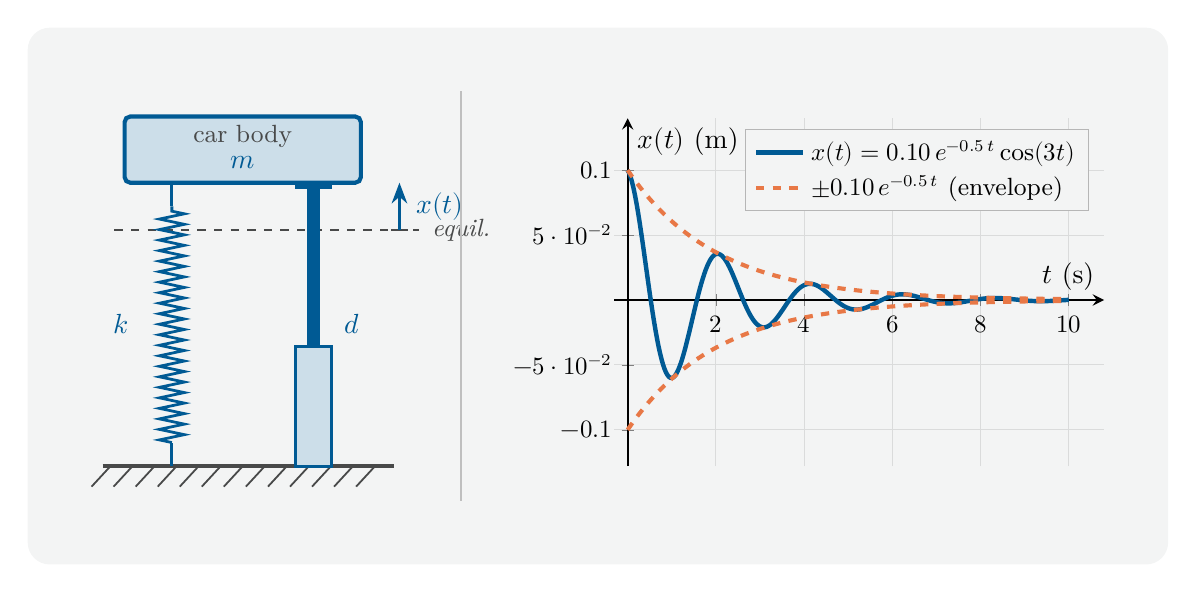
\begin{tikzpicture}[
    show background rectangle,
    background rectangle/.style={fill=my_lightgray, rounded corners=8pt},
    inner frame sep=0.8cm
]

% ─────────────────────────────────────────────────────────────────────────────
% LEFT PANEL  –  mechanical sketch
% Coordinate system: ground at y = 0, positive y upward.
% Car body is drawn slightly above equilibrium (y = 3.0 cm) to make
% the x(t) indicator arrow visible.
% ─────────────────────────────────────────────────────────────────────────────

% Ground line
\draw[my_darkgray, line width=1.5pt] (0.50, 0) -- (4.20, 0);

% Ground hatching (standard fixed-support symbol)
\foreach \xh in {0.60, 0.88, 1.16, 1.44, 1.72, 2.00,
                  2.28, 2.56, 2.84, 3.12, 3.40, 3.68, 3.96}
    \draw[my_darkgray, line width=0.65pt]
        (\xh, 0) -- (\xh - 0.24, -0.26);

% Equilibrium reference line (dashed)
\draw[my_darkgray, line width=0.65pt, dashed]
    (0.65, 3.00) -- (4.52, 3.00);
\node[right, font=\small\itshape, text=my_darkgray] at (4.56, 3.00)
    {equil.};

% ── Spring (left, centre-x = 1.38) ──────────────────────────────────────────
% Short straight lead-in from ground attachment
\draw[my_darkblue, line width=1pt] (1.38, 0.00) -- (1.38, 0.30);
% Zigzag coils
\draw[my_darkblue, line width=1pt,
      decorate, decoration={zigzag, segment length=3.8pt, amplitude=4.5pt}]
    (1.38, 0.30) -- (1.38, 3.30);
% Short straight lead-out to car-body bottom
\draw[my_darkblue, line width=1pt] (1.38, 3.30) -- (1.38, 3.60);
% Label k
\node[left, font=\itshape, text=my_darkblue, inner sep=2pt]
    at (0.90, 1.80) {$k$};

% ── Damper / viscous dashpot (right, centre-x = 3.18) ───────────────────────
% Outer cylinder (fixed to ground)
\draw[fill=my_lightblue, draw=my_darkblue, line width=1pt]
    (2.95, 0.00) rectangle (3.41, 1.52);
% Inner rod (attached to car body, slides in cylinder)
\draw[fill=my_darkblue, draw=my_darkblue, line width=0pt]
    (3.10, 1.52) rectangle (3.26, 3.60);
% Cap at car-body attachment point
\draw[fill=my_darkblue, draw=my_darkblue, line width=0pt]
    (2.95, 3.52) rectangle (3.41, 3.60);
% Label d
\node[right, font=\itshape, text=my_darkblue, inner sep=2pt]
    at (3.50, 1.80) {$d$};

% ── Car body ─────────────────────────────────────────────────────────────────
\draw[fill=my_lightblue, draw=my_darkblue, line width=1.5pt,
      rounded corners=2pt]
    (0.78, 3.60) rectangle (3.78, 4.44);
% "car body" text
\node[font=\small, text=my_darkgray] at (2.28, 4.19) {car body};
% Mass label m
\node[font=\itshape, text=my_darkblue] at (2.28, 3.86) {$m$};

% ── x(t) displacement indicator ─────────────────────────────────────────────
% Tick mark at equilibrium level
\draw[my_darkgray, line width=1pt] (4.16, 3.00) -- (4.38, 3.00);
% Arrow from equilibrium to car-body bottom  (marker-end = Stealth arrowhead)
\draw[my_darkblue, line width=1pt, -Stealth]
    (4.27, 3.00) -- (4.27, 3.60);
% Label x(t)
\node[right, font=\itshape, text=my_darkblue]
    at (4.36, 3.30) {$x(t)$};

% Panel separator
\draw[my_darkgray!35, line width=0.5pt] (5.05, -0.44) -- (5.05, 4.76);

% ─────────────────────────────────────────────────────────────────────────────
% RIGHT PANEL  –  graph of x(t) = 0.10 e^{-0.5 t} cos(3 t)
% ─────────────────────────────────────────────────────────────────────────────

\begin{axis}[
    % Position the south-west corner of the complete axis node
    at={(7.0cm, -0.0cm)},
    anchor=south west,
    width=7.80cm,
    height=6.00cm,
    % Centre-crossing axes
    axis lines=center,
    axis line style={thick},
    % Domain and range
    xmin=-0.30, xmax=10.80,
    ymin=-0.128, ymax=0.140,
    % Labels
    xlabel={$t$~(s)},
    ylabel={$x(t)$~(m)},
    % Ticks (origin label omitted to avoid crowding at the intersection)
    xtick={2, 4, 6, 8, 10},
    ytick={-0.10, -0.05, 0.05, 0.10},
    tick label style={font=\small},
    % Grid
    grid=both,
    grid style={line width=0.3pt, draw=my_darkgray!20},
    % Legend
    legend pos=north east,
    legend style={font=\small, fill=my_lightgray, draw=my_darkgray!40},
    legend cell align=left,
]

% Displacement  x(t) = 0.10 e^{-0.5 t} cos(3 t)
% Note: pgfplots trig functions expect degrees, so cos(3t rad) = cos(deg(3x))
\addplot[
    draw=my_darkblue,
    samples=300,
    ultra thick,
    domain=0:10
]{ 0.10 * exp(-0.5*x) * cos(deg(3*x)) };
\addlegendentry{$x(t) = 0.10\,e^{-0.5\,t}\cos(3t)$}

% Upper exponential envelope  +A e^{-delta t}
\addplot[
    draw=my_orange,
    line width=1.5pt,
    dashed,
    domain=0:10,
    samples=120
]{ 0.10 * exp(-0.5*x) };
\addlegendentry{$\pm 0.10\,e^{-0.5\,t}$ (envelope)}

% Lower exponential envelope  -A e^{-delta t}
% No separate legend entry: covered by the \pm in the entry above
\addplot[
    draw=my_orange,
    line width=1.5pt,
    dashed,
    domain=0:10,
    samples=120
]{ -0.10 * exp(-0.5*x) };

\end{axis}

\end{tikzpicture}
\end{document}
